
\documentclass[11pt,a4paper,sans]{moderncv}        % possible options include font size ('10pt', '11pt' and '12pt'), paper size ('a4paper', 'letterpaper', 'a5paper', 'legalpaper', 'executivepaper' and 'landscape') and font family ('sans' and 'roman')

% moderncv themes
\moderncvstyle{classic}                            % style options are 'casual' (default), 'classic', 'oldstyle' and 'banking'
\moderncvcolor{blue}                               % color options 'blue' (default), 'orange', 'green', 'red', 'purple', 'grey' and 'black'
%\renewcommand{\familydefault}{\sfdefault}         % to set the default font; use '\sfdefault' for the default sans serif font, '\rmdefault' for the default roman one, or any tex font name
%\nopagenumbers{}                                  % uncomment to suppress automatic page numbering for CVs longer than one page


\makeatletter
\renewcommand*{\bibliographyitemlabel}{\@biblabel{\arabic{enumiv}}}
\makeatother

% adjust the page margins
\usepackage[scale=0.76]{geometry}
\setlength{\hintscolumnwidth}{2.05cm}                % if you want to change the width of the column with the dates
%\setlength{\makecvtitlenamewidth}{10cm}           % for the 'classic' style, if you want to force the width allocated to your name and avoid line breaks. be careful though, the length is normally calculated to avoid any overlap with your personal info; use this at your own typographical risks...

%%%%%%%%%%%%%% Nasty hack to avoid whitespace before the bib
\makeatletter
\renewenvironment{thebibliography}[1]{%
%     \section*{\refname}%
%      \@mkboth{\MakeUppercase\refname}{\MakeUppercase\refname}%
      \list{\@biblabel{\@arabic\c@enumiv}}%
           {\settowidth\labelwidth{\@biblabel{#1}}%
            \leftmargin\hintscolumnwidth
            \advance\leftmargin\labelsep
            \@openbib@code
            \usecounter{enumiv}%
            \let\p@enumiv\@empty
            \renewcommand\theenumiv{\@arabic\c@enumiv}}%
      \sloppy
      \clubpenalty4000
      \@clubpenalty \clubpenalty
      \widowpenalty4000%
      \sfcode`\.\@m}
     {\def\@noitemerr
       {\@latex@warning{Empty `thebibliography' environment}}%
      \endlist}
\makeatother

\usepackage[normalem]{ulem}
\usepackage{color}
\usepackage{bm}
\usepackage{amstext}
\usepackage{amssymb}
\newcommand{\coloredLink}[2]{\textcolor{blue}{\href{#1}{#2}}}
\usepackage{tikzpagenodes}


\newcommand\ttbb{\ensuremath{t\bar{t}b\bar{b}}}
\newcommand\ttbar{\ensuremath{t\bar{t}}}
\newcommand\tttt{\ensuremath{t\bar{t}t\bar{t}}}
\newcommand\ttH{\ensuremath{t\bar{t}H}}
\newcommand\ttZ{\ensuremath{t\bar{t}Z}}
\newcommand\ttW{\ensuremath{t\bar{t}W}}
\newcommand\bbbar{\ensuremath{b\bar{b}}}
\newcommand{\met}{\ensuremath{E_{{T}}^{{miss}}}}
\newcommand{\pt}{\ensuremath{p_{T}}}

\newif\ifAddReferences  %% References
\newif\ifAddStatement  %% Statement of research interest
\newif\ifAddInternalTalks  %% References
\newif\ifAddTalks  %% References
\AddReferencesfalse
\AddStatementfalse
\AddInternalTalksfalse
\AddTalkstrue

\AtBeginDocument{\hypersetup{colorlinks,citecolor=blue,linkcolor=blue,urlcolor=blue}}
\AtBeginDocument{\renewcommand\refname{~}}

\name{Javier}{Montejo Berlingen} %many FIXME around the CV, find them
%%%%%%%%%%%%%%%%%%%%%%
% SINCE YOU ARE READING THIS, LET ME REMIND YOU ABOUT THE IDEA OF HAVING A VERTICAL LINE IN THE MIDDLE
% AND THE RESULTS AND POSITIONS ON BOTH SIDES TO GIVE CONTEXT OF THE TIMELINE
%                                                                  CHECK 'CV nuevo layout.key' <----------
%%%%%%%%%%%%%%%%%%%%%%
\title{CERN Staff Physicist}                               % optional, remove / comment the line if not wanted
%\address{CERN 40/5-C11}{1217 Meyrin}{Switzerland}
%\phone[fixed]{+41~786314562}
%\email{jmontejo@cern.ch}                               % optional, remove / comment the line if not wanted


\usepackage{multibib}
\newcites{article,confnote,proceedings}{{Articles},{Conference Notes},{Proceedings}}


%----------------------------------------------------------------------------------
%            content
%----------------------------------------------------------------------------------
\begin{document}
%-----       resume       ---------------------------------------------------------
\makecvtitle
\vspace*{-15mm}

\begin{tikzpicture}[remember picture,overlay,shift={(current page.north east)}]
\node[anchor=north east,xshift=-2cm,yshift=-2.3cm]{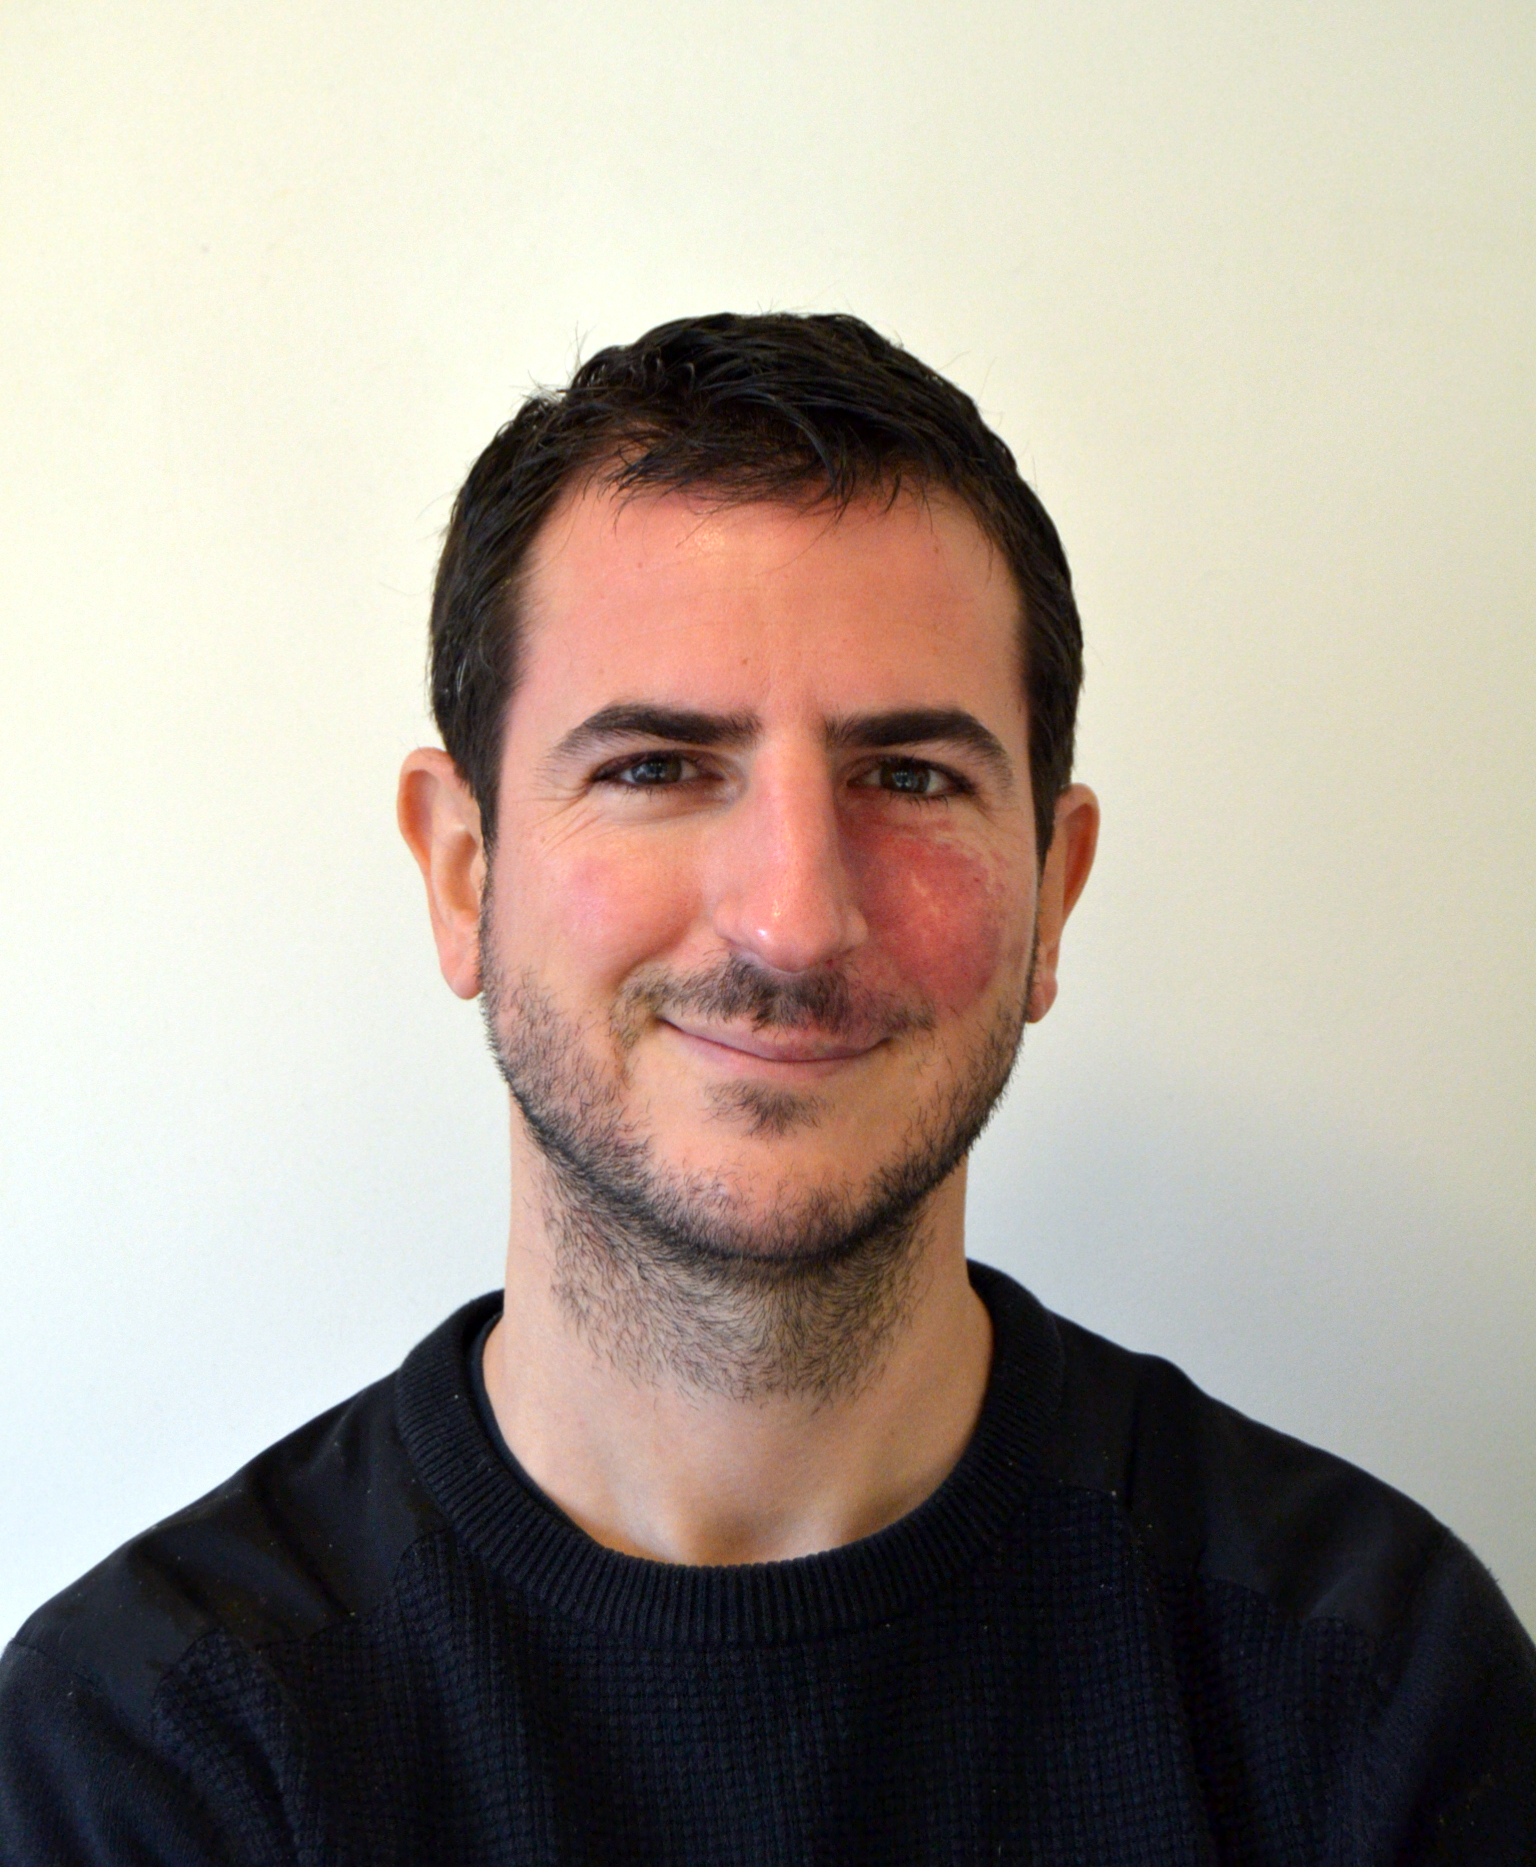
\includegraphics[width=5cm]{Javi_foto_curriculum_gimp_crop}};
\end{tikzpicture}

\section{Personal Information}
\cvline{Date of birth}{March 26, 1986}
%\cvline{Place of birth}{Salamanca, Spain}
%\cvline{Sex}{Male}
\cvline{Nationality}{Spanish, German}
\cvline{Email}{jmontejo@cern.ch}
\cvline{Phone}{+41 786314562}

\vspace*{5mm}




\section{Education and Research Positions}
\cventry{2017 - today}{CERN Staff Physicist}{}{}{
\newline{}SUSY R-parity violating and long-lived subgroup convener.
\newline{}Trigger Level-1 calorimeter algorithm and performance coordinator.
\newline{}Trigger menu coordinator.
\newline{}Scientific secretary for the Trigger Coordination Group.
\newline{}Supervisor to two CERN fellows.}{}
\cventry{2015 - 2017}{CERN Fellow}{}{}{\newline{}SUSY third-generation subgroup convener.}{}
\cventry{2012 - 2015}{Ph.D.,}{Universitat Aut\'onoma de Barcelona,}{Spain.}{\newline{}
ATLAS thesis award.\newline{}Springer thesis award.}{}
\cventry{2011 - 2012}{M.Sc. in High-Energy Physics,}{Universitat Aut\'onoma de Barcelona,}{Spain.}{}{}
\cventry{2005 - 2011}{B.Sc. in Computer Science,}{Universidad de Salamanca,}{Spain.}{\newline{}
Extraordinary Graduation Award.}{}
\cventry{2005 - 2010}{B.Sc. in Physics,}{Universidad de Salamanca,}{Spain.}{\newline{}Extraordinary Graduation Award.\newline{}National Award for Excellence in Academic Performance.}{}{}

\section{Outreach} %FIXME
\cvitem{}{Beamline for schools (B4LS) 2020, assistant and analysis support.}
\cvitem{}{International masterclass 2016--2018, moderator and virtual visits.}
\cvitem{}{World of work 2018, host and supervisor.}
\cvitem{}{ATLAS guide since 2015.}


\ifAddStatement
\clearpage
%\setlength{\hintscolumnwidth}{0cm}
%\setlength{\maincolumnwidth}{15.6cm}
\section{Statement of research interest}
\cvitem{}{
After the successful observation of the Higgs boson in Run 1, the increased energy of Run 2 has provided the LHC experiments with an unprecedented dataset to explore the energy frontier. No significant excess has been observed so far, and stringent limits have been set on simplified models. 
The motivation for some form of new physics is still strong but it is obvious that it is not manifested in the vanilla signatures that were the main focus of attention. 
At this stage two different approaches can and should be pursued. On one side, searches in final states with low cross section or challenging signatures will become more relevant with the growing dataset. On the other side, precision measurements are critically needed and are extremely valuable results on their own. 
Especially important are measurements in final states with non-zero electric charge, since they can not be measured at future electron-positron colliders. 
}

\cvitem{}{
The ATLAS measurement program has been extremely successful, and processes with cross-sections as low as $\mathcal{O}(1)$ fb have been measured. However it is important to keep in mind that so far less than 5\% of the target of 3000 $\text{fb}^{-1}$ has been recorded. The large increase in luminosity will benefit especially processes with low cross-sections, and final states with high purity but low branching ratios, such as multi-lepton final states. In addition, it will also transform the treatment of objects where the choice of working point means a trade-off between purity and statistics. Examples of such are identification and isolation of leptons, or tagging of jets originating from $b$-quarks ($b$-jets). 
%Another example based on an ATLAS analysis is the current \ttH\ multi-lepton analysis, which has a background from fake or non-prompt lepton that accounts for about 40\% of the observed events in many of its best signal regions. Handles to suppress these reducible backgrounds exist but the low number of signal events requires an analysis with high acceptance. There is also non-negligible diboson background, which contains prompt isolated leptons but enters the analysis region mostly via mis-tagged jet, with only a small contribution from diboson plus heavy flavour jets. Both backgrounds 
}
\cvitem{}{
For the aforementioned reasons, I consider that a program of measurements in final states with multiple leptons and $b$-jets will become extremely valuable during the next years, and up to the high-luminosity phase of LHC (HL-LHC). 
}

%multilepton multib
%ttW measurement
%W+bb
%soft muon top mass???
%need something also more longer term
% ttW
\cvitem{ttW}{
One of the processes that has been measured for the first time at the LHC is the \ttW\ process. Several ATLAS results at 8 and 13 TeV have measured \ttW\ cross-sections which deviate from the SM prediction, and a better understanding of this process is essential. 
In particular unexpected correlations of the charge asymmetry with the jet and $b$-jet multiplicity are observed consistently, which require further study. 
Unfolded measurements of kinematic variables will be provided in the short future, however there are several reasons why a measurement of this process will be dramatically improved with the increase in luminosity of upcoming years:
\begin{itemize}
\item The increase of statistics will allow for an analysis with a tighter lepton identification and isolation, which could reduce to a negligible level the background from fake and non-prompt leptons, almost doubling the signal purity in several regions. The remaining background originates mostly from \ttZ\ with a lost lepton, which can be measured very precisely.
\item Given the unexpected correlations seen with the charge asymmetry, 2-dimensional measurements of the charge asymmetry with the number or jets, or number of $b$-jets, will be required to study this effect. Such multi-dimensional measurements are not possible without higher luminosity.
\end{itemize}
}
\cvitem{}{
\begin{itemize}
\item A requirement of two $b$-tags in the event (currently restricted to one $b$-tag) will reduce the combinatorial problem when pairing leptons and jets to build observables closely related to top-quark kinematics. It will also allow a cleaner measurement of the production of additional jets, especially in the three-lepton category. Improving the resolution of the measurement, and reconstructing correctly observables that link directly to the top quark kinematics, are critical improvements in a final state where the presence of multiple neutrinos prevents the full reconstruction exploiting the known mass constraints.
\end{itemize}
As discussed, the larger dataset of the HL-LHC will certainly benefit most of the analyses, but it has the potential to really transform the \ttW\ measurement.
}

% V+bb
\cvitem{W+bb}{
%\cvitem{\textbf{}}{}{}{}{
The measurement of a $W$ boson in association with $b$-jets is an extremely challenging one due to the massive background from \ttbar\ production. The lepton charge asymmetry can be exploited to separate out this process, however it is then again drowned by single-top production in $t$-channel, which produces a similar final state with a $W$-boson, $b$-jets, and is also charge asymmetric. These challenges have led to only one ATLAS measurement of this process, at 7 TeV measuring the inclusive $W$+b cross-section, and a differential measurement of $W$+b together with single top.
This process represents also the main background to $WH(b\bar{b})$, and becomes increasingly relevant now that Higgs measurement move towards the measurement of simplified template cross-sections at high $p_T(H)$, leading to close-by $b$-jets. In this topology the contribution of $W$+bb, where the $b$-jet pair originates from gluon splitting, is strongly enhanced while the \ttbar\ background is suppressed given that the $b$-jets tend to be aligned back-to-back. This collinear regime carries an additional intrinsic interest since MC generators are usually not able to model it correctly.
}
\cvitem{}{
%Valuable by itself, probe of gluon fragmentation. Largely unconstrained at small opening angles
I am interested in a measurement of the $W$+bb process, focusing in the regime with two close-by $b$-jets. In order to overcome the intrinsic limitation of the radius of R=0.4 that is used in jet reconstruction, the measurement would be performed with muons produced in B-hadron decays. In particular selecting two same-sign muons in addition to the lepton from the $W$ boson provides a number of extremely interesting benefits:
\begin{itemize}
\item No intrinsic limitation in $\Delta R$ space, compared to the limit of $\Delta R=0.4$ in jets, or $\Delta R=0.2$ in track-jets. The superb spatial resolution of muons allows to probe a regime that has not been measured before
\item The study of the collinear regime provides a natural suppression of the \ttbar\ background. Based on MC studies the \ttbar\ background is expected to be less than 10\% of the signal.
\item A common limitation to measurements of heavy flavour production is the precise determination of the additional heavy-flavour backgrounds such as single $b$-jet with an additional mistagged jet, or pairs of charm jets. The requirement of muons with same electric charge can only be satisfied in events with two B-hadrons, where the first muon comes from a semileptonic B-hadron decay, and the second from a cascade of B-hadron to D-hadron and subsequent leptonic decay. Muon pairs from single B-hadron or two D-hadrons can only produce opposite-sign muons, except for rare cases of D-hadron oscillations.
\item The full event selection and measurement can be performed purely based on lepton observables, leading to a measurement with extremely low systematic uncertainties. 
\end{itemize}
}
\cvitem{}{
\begin{itemize}
\item A natural evolution of the analysis is the transition from two muons from the B-hadron decays, to two $J/\psi\rightarrow\mu\bar{\mu}$ decays. The extremely low branching ratio (BR($B\rightarrow J/\psi\rightarrow\mu\bar{\mu}=5\cdot 10^{-4}$) would not be an obstacle at HL-LHC, and provides an even cleaner final state with improved spatial correspondence between the B-hadron direction and the measured $J/\psi$.
\end{itemize}
}

\cvitem{}{
In addition, an analysis in this final state would have a large synergy with future top mass measurements exploiting the same $B\rightarrow J/\psi\rightarrow\mu\bar{\mu}$ decay, as way of avoiding the systematic uncertainties due to jet energy calibration and $b$-tagging.
}

%% ML
\cvitem{ML for lepton id.}{
While the increase in luminosity allows for a natural tightening of the lepton identification and isolation criteria, a high efficiency is in many cases still desirable, in order to minimise systematic uncertainties due to efficiency corrections. The rapid evolution of the machine-learning (ML) field has provided a magnificent set of tools that can be applied in high energy physics to boost the performance in multiple areas. In particular improvements to lepton identification and isolation will have a positive benefit to the full ATLAS program.
}
\cvitem{}{
Basic multi-variate techniques have been applied to electron identification, such as likelihood discriminants, based on crafted high-level features. Muon identification in the regime of interest for $W$-boson decays is based on simple cuts on a set of variables.
The potential for improvements is immense, and a targeted program in this area would bring a wide range of improvements.
\begin{itemize}
\item The set of variables used for identification can be extended to incorporate low-level data at the level of tracks or individual cells via convolutional neural networks. The inclusion of low-level features in addition to high-level features selected by physicist has been shown to consistently improve the separation in classification tasks.
\item The usage of a simple likelihood technique in electron identification, which neglects useful variable correlations, has its motivation in the poor modelling of MC simulation of electron shower shapes. This problem could become even more severe with the introduction of additional low-level features. A switch in paradigm would be required in order to train the ML discriminants directly on data, exploiting leptonic $Z$ decays via tag-and-probe, which provides a clean sample of unbiased leptons.
\item A certain mixture of backgrounds are the target of different requirements in the selection process. For example the electron identification aims at rejecting jets, isolation provides an additional rejection for non-prompt electrons, which might be followed by a material conversion veto, and electron charge misidentification. The factorisation of these steps is not always obvious, and changes to one of the criteria might strongly affect the performance of further steps. A unified approach where all steps are combined into a single multi-class classifier is a promising approach, where the optimal selection over the full set of backgrounds can be determined. A single criteria for identification plus isolation would in addition have access to information about the correlation of both, providing useful additional information towards the rejection of backgrounds.
\end{itemize}
}
\cvitem{}{
The modernisation of lepton identification and isolation selection has the potential to improve the performance of essential objects for the whole collaboration such as leptons. However the relatively straightforward application of modern techniques has to be carefully balanced against our capabilities to calibrate successfully the resulting selection. Such calibration and the tuning of a `lepton working point` would become tightly linked to the multi-lepton program.
}

%%need to fill a page of VIM in full screen...
%ML lepton identification + isolation
\cvitem{}{
As discussed, I consider that a program of measurements in final states with multiple leptons and $b$-jets has a large potential. In addition it provides the flexibility to fully exploit the fast increase in recorded dataset during the next years, and up to HL-LHC.
}

%\setlength{\hintscolumnwidth}{2.05cm}
\fi

\clearpage
\section{Research Experience}

%%%%%%%%%%%%%%%% ttH(bb)
\cvitem{{Run~1: t\=tH(b\=b)}}{
At the beginning of my PhD, the Higgs boson had recently been discovered, but most of its properties remained to be measured, in particular the couplings to quarks.
I decided to concentrate on the associated production of a Higgs boson and a top quark pair (\ttH), given the important role of top Yukawa coupling which, due to the loop corrections to the Higgs mass, is the main contributor to the hierarchy problem.
%is the only ``natural'' Yukawa coupling, with $\lambda_\text{t}\approx 1$.
%Measuring the top Yukawa via the \ttH\ production cross section also provides a handle to identify possible BSM contributions in the dominant Higgs production mode, which is the loop-induced gluon-gluon fusion process, and also the very sensitive decay to two photons.
%In addition, due to the loop corrections to the Higgs mass, the top Yukawa coupling is the main contributor to the hierarchy problem.
}
\cvitem{}{
In order to compensate the low \ttH\ production cross section, I decided to target the decay of the Higgs boson to \bbbar\ and semileptonic \ttbar\ decay.
I focused on the development of the selection, fitting strategy and background estimation.
In particular the challenging \ttbb\ background modelling and associated systematic uncertainties.
A collaboration with theorists was started to improve the modelling of \ttbb\ to NLO for the first time. I worked in the integration of this improved modelling in the \ttbb\ subset within the inclusive \ttbar+jets sample, via a multi-dimensional reweighting.
}
\cvitem{}{
The results of the \ttH\ analysis were summarised in publications at 7 TeV~\cite{ATLAS-CONF-2012-135}, and 8 TeV~\cite{HIGG-2013-27}. The analysis was included in the ATLAS Higgs coupling combination~\cite{HIGG-2014-06}, and further combined with CMS~\cite{HIGG-2015-07}, leading to the first evidence of \ttH\ production under the assumption of SM branching ratios.
}

%%%%%%%%%%%%%%%%% BSM ttbb
\cvitem{{Run~1: BSM t\=tb\=b}}{
The confirmation of the SM-like nature of the top Yukawa coupling (at least to first order), implied also the corroboration of large loop corrections to the Higgs mass, leading to the hierarchy problem. I decided to explore BSM signatures in the \ttbb\ final state, that could provide solutions to the hierarchy problem via fermionic top partners (vector-like quarks, VLQ) or bosonic top partners (stops) cancelling the contribution from top quarks. Both searches involved a full redesign of the previous \ttH(bb) analysis, tailoring the selection and fitted variables to the considered signals. 
}
\cvitem{}{
The search for VLQ decaying to a Higgs boson and a top quark ($T\rightarrow H t$) required to improve the understanding of the \ttbb\ background in the high-energy and boosted regime. The analysis included for the first time combinations with other VLQ searches and set limits on the VLQ mass regardless of its decay branching ratios~\cite{EXOT-2013-18}.
}
\cvitem{}{
The second search targeted supersymmetric models were the mass difference between the lightest stop and neutralino is close to the top mass, where existing searches had no sensitivity. The search exploits the production of the heavier stop and the subsequent decay to the lightest stop and neutralino ($\tilde{t}_2 \rightarrow \tilde{t}_1 H$). The presence of additional \met\ allows to suppress backgrounds, but increases the importance of previously subdominant backgrounds such as dileptonic \ttbb\ with one lost lepton.
The results of the search~\cite{SUSY-2014-07}, were combined with existing searches in complementary decay channels ($\tilde{t}_2 \rightarrow \tilde{t}_1 Z$, and $\tilde{t}_2 \rightarrow t \tilde{\chi}^0_1$), to provide limits on the stop mass regardless of its decay.
}

\cvitem{Run~1: Tile calorimeter}{During my PhD I  also worked on the characterisation and calibration of the timing performance of the Tile calorimeter using collision data. I identified multiple detector and geometrical effects that were previously not accounted for, and introduced a set of selection cuts and corrections that improved the resolution of the time measurement up to 20\%~\cite{TCAL-2017-01}.
}
\cvitem{}{
I also gained some hardware experience by contributing to the maintenance and repairs of modules during the LS1 phase.
After my work on the calorimeter performance I contributed as Data Quality Validator and Data Quality Leader for the Tile calorimeter.
}

\cvitem{{Run~2: RPC SUSY}}{
The large increase in energy and luminosity at the start of Run~2 made it the perfect moment to embark on BSM searches, which would benefit the most from the increased centre-of-mass energy. 
As one of the prime candidates to address the hierarchy problem, I focused on searches for supersymmetry, in particular I joined the search for top squarks in the single-lepton final state.
%My focus was on the challenging regions of phase-space where top squarks with masses well below 1 TeV were not excluded. 
}
\cvitem{}{
I redesigned the background estimation techniques used in the search in order to reduce the reliance on MC simulation, and developed new selections to further suppress backgrounds.
The optimised selection increased the relevance of previously subdominant backgrounds with large uncertainties, such as $\ttZ(\nu\bar{\nu})$ or single top, for which I developed dedicated control regions.
I also contributed to the design of new signal benchmarks, moving away from simplified models in favour of more complex scenarios inspired by feasible and promising pMSSM benchmarks.
One such example is the production of stop pairs with decay to higgsinos, featuring small splittings, and leading to a final state with soft leptons ($\lesssim 5$ GeV) which is experimentally challenging.
The strong sensitivity and flexibility of the analysis led to a series of publications with 3.2~fb$^{-1}$\cite{SUSY-2015-02}, 14 fb$^{-1}$\cite{ATLAS-CONF-2016-050} and 36 fb$^{-1}$\cite{SUSY-2016-16}, with increasingly comprehensive coverage of stop production within natural SUSY scenarios.
}
\cvitem{}{
During this period I was appointed as convener of the third-generation SUSY subgroup, where I managed to bring to a timely completion the program of searches with 36~fb$^{-1}$, and lead the preparation of analyses for the full Run 2 results. I initiated a restructuring of the analysis groups to merge searches for third-generation squarks and searches for dark matter with associated heavy-flavour quarks, leading to stronger and better organised teams that delivered impressive results on both models.
}

\cvitem{{Run~2: RPV SUSY}}{
Although supersymmetry is a very compelling extension of the SM, no hints for vanilla SUSY has been observed. This motivates the extension of the searches to less traditional final states. I have developed a completely new search for RPV SUSY in final states with no missing transverse energy (\met), at least one lepton and high number of jets (up to 15 jets and 4 $b$-jets). The absence of \met\ in the final state is a feature that could cause supersymmetric particles to remain unobserved due to the large requirements on \met\ placed by most searches. The background modelling at very high jet multiplicities is extremely challenging, and I developed new data-driven methods to estimate the background. The first iterations of the search focused on strong production of gluinos and stops, and set stringent exclusion limits on models that were previously completely uncovered~\cite{ATLAS-CONF-2016-094, SUSY-2016-11}. Due to its design as model-independent search, I also contributed to the reinterpretation of the search in dark matter models yielding four-top production~\cite{EXOT-2017-32}.
}
\cvitem{}{
The analysis with full Run 2 data had as target benchmark higgsino production. In order to reach sensitivity to such low cross sections I introduced machine-learning techniques, where custom modifications of the loss function allows the discriminant to be invariant with respect to the number of $b$-jets. This property is exploited to extend the data-driven background estimation to the shape of the discriminant. The sensitivity of the analysis is strongly increased with no additional reliance on MC. 
The search reaches sensitivity to higgsino production with RPV decay to quarks~\cite{ATLAS-CONF-2021-007}, and is the first analysis to surpass the limits from LEP.
%Highlighted in the CERN courier https://cerncourier.com/wp-content/uploads/2021/04/CERNCourier2021MayJun-digitaledition.pdf
}
\cvitem{}{
I am currently appointed as convener of the RPV and long-lived SUSY subgroup. During my term I have proposed several analyses in previously unexplored final states, which are now being developed. I have also initiated a task-force to explore the interplay of RPC analyses, prompt RPV analyses, and long-lived searches when considering models where the lifetime of the lightest supersymmetric stable could range from prompt, long-lived, or collider-stable. In this context I coordinated the work in collaboration with performance groups to develop recommendations for the uncertainties on lepton, jet, $b$-jet and \met\ calibrations, when reconstructing slightly long-lived decays. The results showed explicitly for the first time the good coverage provided across the lifetime range of the different analyses, and also highlighted some sensitivity gaps where dedicated searches would be needed~\cite{ATLAS-CONF-2018-003}.
}

\cvitem{Run~2: Trigger}{
I have contributed to the ATLAS trigger menu group throughout Run~2, initially as trigger menu expert and menu on-call, and during 2018--2019 as trigger menu and signature coordinator. As such, I was in charge of coordinating the work of all the signature, detector and physics trigger groups, which encompassed about a hundred members. In this role I was part of the Physics Coordination group, given its critical relevance on the ATLAS physics program. 
During this time I was in charge of defining the menus for the intense period of special runs in 2018, including low-$\mu$, high-$\beta^*$, and the Heavy-Ion run. I was also responsible for the documentation of the trigger menu evolution in dedicated public notes~\cite{ATL-DAQ-PUB-2018-002, ATL-DAQ-PUB-2019-001}.
After the data-taking period I defined the ATLAS physics menu for Run~3~\cite{Run3menu}. I successfully argued for a strongly increased recording rate for Run 3, which was endorsed by the experiment. Besides the menu composition, I contributed to dedicated studies in order to ensure that the trigger menu being designed would respect all the hardware and cabling constraints of the upgraded systems.
}
\cvitem{}{As part of my effort to improve the Run~3 triggers, I am currently Level-1 calorimeter algorithm and trigger performance coordinator.  I am leading the development and optimization of reconstruction and identification algorithms that can maximise the performance and rate gains from the upgraded calorimeters, exploiting the capabilities of the new system to its full potential.
}


\clearpage
%\section{List of publications}
\cvitem{}{Highlighted in bold are the three publications that I attach as the most significant ones.}

\cvitem{Run~1: ttH(bb)}{
I was one of the main analysers in the first ATLAS analysis targeting the \ttH\ production mode, contributing to the development of the selection, fitting strategy and background estimation. In particular the challenging \ttbb\ background modelling and associated systematic uncertainties, where a collaboration with theorists was started. I studied the \ttbb\ modelling for the first time at NLO, and integrated the dedicated calculation in the inclusive \ttbar+jets sample via a multi-dimensional reweighting.
\begin{itemize}
\item Search for the Standard Model Higgs boson produced in association with top quarks in proton-proton collisions at $\sqrt{s}=7$ TeV using the ATLAS detector~\cite{ATLAS-CONF-2012-135}.
\item \textbf{Search for the Standard Model Higgs boson produced in association with top quarks and decaying into $b\bar{b}$ in pp collisions at $\sqrt{s}=8$ TeV with the ATLAS detector}~\cite{HIGG-2013-27}. 
\item Measurements of the Higgs boson production and decay rates and coupling strengths using pp  collision data at $\sqrt{s}=7$ and 8 TeV in the ATLAS experiment~\cite{HIGG-2014-06}.
\item Measurements of the Higgs boson production and decay rates and constraints on its couplings from a combined ATLAS and CMS analysis of the LHC pp collision data at $\sqrt{s}=7$ and 8 TeV~\cite{HIGG-2015-07}.
\end{itemize}
}

\cvitem{Run~1: BSM ttbb}{
I developed searches for fermionic and bosonic top partners in the \ttbb\ final states. Both searches involved a full redesign of the previous \ttH(bb) analysis, tailoring the selection and fitted variables to the considered signals. For both analyses I was the main (and only) analyser, together with my supervisor.
\begin{itemize}
\item Search for production of vector-like quark pairs and of four top quarks in the lepton-plus-jets final state in pp collisions at $\sqrt{s}=8$ TeV with the ATLAS detector~\cite{EXOT-2013-18}.
\item ATLAS Run 1 searches for direct pair production of third-generation squarks at the Large Hadron Collider~\cite{SUSY-2014-07}.
\end{itemize}
}

\cvitem{Tile calorimeter}{
I worked in the characterisation of the Tile calorimeter timing performance and calibration with muons from collision events.
\begin{itemize}
\item Operation and performance of the ATLAS Tile Calorimeter in Run 1~\cite{TCAL-2017-01}.
\end{itemize}
}

\cvitem{Run~2: RPC SUSY}{
I was analysis contact in the search for top squarks in the single-lepton final state, leading a group of around 15 people. Redesigned the background estimation methods to reduce the reliance on MC simulation, and developed new selections to further suppress backgrounds. I also defined new signal benchmarks, in order explore more comprehensively challenging models with low stop masses.
\begin{itemize}
\item Search for top squarks in final states with one isolated lepton, jets, and missing transverse momentum in $\sqrt{s}=13$ TeV pp collisions with the ATLAS detector~\cite{SUSY-2015-02}.
\item Search for top squarks in final states with one isolated lepton, jets, and missing transverse momentum in $\sqrt{s}=13$ TeV pp collisions with the ATLAS detector~\cite{ATLAS-CONF-2016-050}. 
\item \textbf{Search for top-squark pair production in final states with one lepton, jets, and missing transverse momentum using 36 fb$^{-1}$ of $\sqrt{s}=13$ TeV pp collision data with the ATLAS detector}~\cite{SUSY-2016-16}.
\end{itemize}
}

\cvitem{Run~2: RPV SUSY}{
I co-designed with another CERN fellow a fully new analysis targeting the final state of a lepton plus many jets (up to 15 jets and 4 $b$-jets), which was previously uncovered. The main challenge was the background estimation at these extreme multiplicities for which we developed fully new data-driven methods. I am also paper editor for the full Run 2 paper. Due to its wide applicability I also contributed to its reinterpretation in four-top models, and SUSY models with displaced decays, where I was also CONF editor.
\begin{itemize}
\item Search for new phenomena in a lepton plus high jet multiplicity final state with the ATLAS experiment using $\sqrt{s}=13$ TeV proton-proton collision data~\cite{SUSY-2016-11}.
\item \textbf{Search for R-parity violating supersymmetry in a leptons plus high jet multiplicity final state with the ATLAS experiment using 139 fb$^{-1}$ of $\sqrt{s}=13$ TeV proton--proton collision data}~\cite{RPV1L} (in approval).
\item Constraints on mediator-based dark matter and scalar dark energy models using $\sqrt{s}=13$ TeV pp collision data collected by the ATLAS detector~\cite{EXOT-2017-32}.
\item Reinterpretation of searches for supersymmetry in models with variable R-parity-violating coupling strength and long-lived R-hadrons~\cite{ATLAS-CONF-2018-003}.
\end{itemize}
}


\cvitem{Trigger}{
I was editor of the 2017 trigger menu PUB note, and coordinator and supervisor of the 2018 trigger menu PUB note. I also was in charge of the design of the Run 3 trigger menu.
\begin{itemize}
\item Trigger Menu in 2017~\cite{ATL-DAQ-PUB-2019-001}.
\item Trigger Menu in 2018~\cite{ATL-DAQ-PUB-2018-002}.
\item Run 3 trigger menu design~\cite{Run3menu}.
\end{itemize}
}


\section{List of publications}
\cvitem{}{A list of the 10 most important publications where I have been the main contributor is given below.}

\cvitem{Run~1: t\=tH(b\=b) and BSM t\=tb\=b}{
Main analyzer for the t\=tH(b\=b), VLQ and $\tilde{t}_2 \rightarrow \tilde{t}_1 H$ analyses. The latter is documented as part of the third-generation squarks summary paper.
\begin{itemize}
\item Search for the Standard Model Higgs boson produced in association with top quarks and decaying into $b\bar{b}$ in pp collisions at $\sqrt{s}=8$ TeV with the ATLAS detector~\cite{HIGG-2013-27}. 
\item Search for production of vector-like quark pairs and of four top quarks in the lepton-plus-jets final state in pp collisions at $\sqrt{s}=8$ TeV with the ATLAS detector~\cite{EXOT-2013-18}.
\item ATLAS Run 1 searches for direct pair production of third-generation squarks at the Large Hadron Collider~\cite{SUSY-2014-07}.
\end{itemize}
}

\cvitem{Tile calorimeter}{
Contributor to the characterisation of the Tile calorimeter timing performance and calibration, documented as part of the Tile Calorimeter paper.
\begin{itemize}
\item Operation and performance of the ATLAS Tile Calorimeter in Run 1~\cite{TCAL-2017-01}.
\end{itemize}
}

\cvitem{Run~2: RPC SUSY}{
Main analyzer, analysis contact and paper editor.
\begin{itemize}
\item Search for top squarks in final states with one isolated lepton, jets, and missing transverse momentum in $\sqrt{s}=13$ TeV pp collisions with the ATLAS detector~\cite{SUSY-2015-02}.
\item Search for top-squark pair production in final states with one lepton, jets, and missing transverse momentum using 36 fb$^{-1}$ of $\sqrt{s}=13$ TeV pp collision data with the ATLAS detector~\cite{SUSY-2016-16}.
\end{itemize}
}

\cvitem{Run~2: RPV SUSY}{
Main analyzer, analysis contact and paper editor.
\begin{itemize}
\item Search for new phenomena in a lepton plus high jet multiplicity final state with the ATLAS experiment using $\sqrt{s}=13$ TeV proton-proton collision data~\cite{SUSY-2016-11}.
\item Search for R-parity violating supersymmetry in a leptons plus high jet multiplicity final state with the ATLAS experiment using 139 fb$^{-1}$ of $\sqrt{s}=13$ TeV proton--proton collision data~\cite{ATLAS-CONF-2021-007}
\item Reinterpretation of searches for supersymmetry in models with variable R-parity-violating coupling strength and long-lived R-hadrons~\cite{ATLAS-CONF-2018-003}.
\end{itemize}
}


\cvitem{Trigger}{
Co-editor.
\begin{itemize}
\item Trigger Menu in 2018~\cite{ATL-DAQ-PUB-2018-002}.
\end{itemize}
}




\ifAddTalks
\clearpage
\ifAddInternalTalks
\section{Conferences, schools and workshops}
\else
\section{Conference talks}
\fi
\cventry{Jun 2021}{Large Hadron Collider Physics (LHCP 2021),}{\sout{Paris},}{Virtual}{\newline{}
    Talk: BSM Higgs decays at ATLAS+CMS
}{}{}
\cventry{Jul 2020}{40th International Conference on High Energy Physics (ICHEP 2020),}{\sout{Prague},}{Virtual}{\newline{}
    Talk: Triggering in the ATLAS experiment
    [\coloredLink{https://cds.cern.ch/record/2728145}{ATL-DAQ-SLIDE-2020-320}] 
    [\coloredLink{https://cds.cern.ch/record/2742661}{Proceedings}] 
}{}{}
\cventry{May 2019}{27th International Conference on Supersymmetry and Unification of Fundamental Interactions (SUSY 2019),}{Corpus Christi,}{Texas}{\newline{}
    Talk: Searches for supersymmetry in R-parity violating signatures at the LHC.
    [\coloredLink{https://cds.cern.ch/record/2676781}{ATL-PHYS-SLIDE-2019-242}]
}{}{}
\ifAddInternalTalks
\cventry{May 2019}{Trigger workshop,}{Elba,}{Italy.}{\newline{}
    Talk: Run-3 baseline menu.}{}{} %https://indico.cern.ch/event/772409/
\cventry{Sep 2018}{TDAQ week,}{Krakow,}{Poland.}{\newline{}
    Talk: Menu considerations for Run 3.}{}{} %https://indico.cern.ch/event/730816
    \fi
\cventry{Jul 2018}{23rd International Conference on Computing in High Energy and Nuclear Physics (CHEP 2018),}{Sofia,}{Bulgaria.}{\newline{}
    Talk: The ATLAS Trigger Menu design for higher luminosities in Run 2. [\coloredLink{https://cds.cern.ch/record/2631630}{ATL-DAQ-SLIDE-2018-500}][\coloredLink{https://cds.cern.ch/record/2645347}{Proceedings}]
}{}{} 
\cventry{May 2018}{(Re)interpreting the results of new physics searches at the LHC (ReINPS2018),}{CERN,}{Geneva}{\newline{}
    Talk: Sensitivity of prompt searches to long-lives particles.
    [\coloredLink{https://cds.cern.ch/record/2319790}{ATL-PHYS-SLIDE-2018-282}]
}{}{}
\ifAddInternalTalks
\cventry{Apr 2018}{Four-tops workshop,}{CERN,}{Geneva}{\newline{}
    Talk: Data-driven methods in lepton+jets searches to evaluate the ttbar+jets and W+jets backgrounds.}{}{}
    \fi
\cventry{May 2017}{Large Hadron Collider Physics (LHCP),}{Shangai,}{China.}{\newline{}
    Talk: Unconventional signatures and RPV supersymmetry. Plenary. [\coloredLink{https://cds.cern.ch/record/2266308}{ATL-PHYS-SLIDE-2017-310}]
 \newline{}
    Poster: The ATLAS Run-2 Trigger Menu for higher luminosities: Design, Performance and Operational Aspects. [\coloredLink{https://cds.cern.ch/record/2265272}{ATL-DAQ-SLIDE-2017-255}] }{}{}
\ifAddInternalTalks
\cventry{May 2017}{ATLAS Exotics \& SUSY workshop,}{Bucharest,}{Romania.}{\newline{}
    Talk: RPV searches in ATLAS.}{}{}
\cventry{Feb 2017}{ATLAS trigger workshop,}{University of Geneva,}{Switzerland.}{\newline{}
    Talk: Trigger rates and processing time. Pileup dependency.}{}{}
\cventry{Oct 2016}{ttH workshop,}{CERN,}{Geneva.}{\newline{}
    Talk: ttH to invisible.}{}{}
\cventry{Sep 2016}{TDAQ week,}{Barcelona,}{Spain.}{\newline{}
    Talk: Trigger menu rates and CPU projections in 2017.}{}{}
\cventry{Apr 2016}{Supersymmetry workshop,}{Sussex,}{UK.}{\newline{}
    Talk: RPV analyses in ATLAS.}{}{}
    \fi
\cventry{Mar 2015}{XXIX Rencontres de Physique de la Vall\'{e}e d'Aoste,}{La Thuile,}{Italy.}{\newline{}
    Talk: Search for the Higgs boson in the ttH production channel using the ATLAS detector. 
    %\newline
     [\coloredLink{https://cds.cern.ch/record/2002318}{ATL-PHYS-SLIDE-2015-073}]
    }{}{}
\ifAddInternalTalks
\cventry{Nov 2014}{ttH workshop,}{CERN,}{Geneva.}{\newline{}
    Talk: Sensitivity projections for ttH.}{}{}
\cventry{Jun 2014}{European School of High-Energy Physics,}{Garderen,}{Holland.}{}{}
\cventry{Sep 2013}{ATLAS Higgs to \bbbar\ workshop,}{Marseille,}{France.}{\newline{}
    Talk: ttbar modelling for VH and ttH.}{}{}
    \fi
\cventry{Aug 2013}{21st International Conference on Supersymmetry and Unification of Fundamental Interactions (SUSY 2013),}{Trieste,}{Italy.}{\newline{}
    Talk: Top quark production in the ATLAS detector of the LHC. \newline
     [\coloredLink{https://cds.cern.ch/record/1596998}{ATL-PHYS-SLIDE-2013-509}]
}{}{}
\ifAddInternalTalks
\cventry{Jun 2013}{ttH workshop,}{CERN,}{Geneva.}{\newline{}
    Talk: tt+jets/bb modelling and systematics in ttH(bb) analyses.}{}{}
    \fi
\cventry{May 2013}{Large Hadron Collider Physics (LHCP 2013),}{Barcelona,}{Spain.}{\newline{}
	Poster: Search for the Standard Model Higgs boson produced in association with top quarks and decaying to $b\bar{b}$ at $\sqrt{s} = 7~TeV$. \newline
	[\coloredLink{https://cds.cern.ch/record/1551958}{ATL-PHYS-SLIDE-2013-298}]% \newline{}
   [\coloredLink{http://www.epj-conferences.org/articles/epjconf/abs/2013/21/epjconf_lhcp2013_20028/epjconf_lhcp2013_20028.html}{Proceedings}]}{}{}
\ifAddInternalTalks
\cventry{Dec 2012}{ATLAS Higgs to \bbbar\ workshop,}{Saint Genis,}{France.}{\newline{}Talk: Statistical procedures and limit setting in Higgs to \bbbar.}{}{}
\cventry{Jul 2012}{Hadron Collider Physics School (HASCO 2012),}{G\"ottingen,}{Germany.}{}{}
\fi
\cventry{Mar 2012}{LHC commissioning,}{CERN,}{Geneva.}{\newline{}Poster: ATLAS detector performance in 2011: calorimeters. \newline
[\coloredLink{https://cds.cern.ch/record/1445591}{ATL-PHYS-SLIDE-2012-154}]}{}{}
\ifAddInternalTalks
\cventry{Sep 2011}{4th International Workshop on Top Quark Physics (TOP 2011),}{Sant Feliu de Guixols,}{Spain.}{}{}
\fi
\fi


\ifAddReferences
\clearpage
\section{References}

\cventry{}{ \textbf{Andreas Hoecker} }{}{\newline
European Organization for Nuclear Research (CERN) \newline
+41 22 76 74787\newline
andreas.hoecker@cern.ch\newline
}{}{}

\cventry{}{ \textbf{Marumi Kado} }{}{\newline
Laboratoire de l'Accelerateur Lineaire (LAL)\newline
+41 22 76 71143\newline
kado@lal.in2p3.fr\newline
}{}{}

\cventry{}{ \textbf{Aurelio Juste Rozas} }{}{\newline
Institut de Fisica d'Altes Energies (IFAE)\newline
+34 93 581 4249\newline
juste@ifae.es\newline
}{}{}

\cventry{}{ \textbf{Brian Petersen} }{}{\newline
European Organization for Nuclear Research (CERN) \newline
+41 22 76 71199\newline
brian.petersen@cern.ch\newline
}{}{}

\cventry{}{ \textbf{Joerg Stelzer} }{}{\newline
University of Pittsburgh\newline
+41 22 76 78979\newline
stelzer@cern.ch\newline
}{}{}

\fi

\end{document}


%% end of file `template.tex'.
